\chapter{First chapter in this}%\label{chap:...}
Chapter description

% Chapters
%\input{part_spring1/somefile}

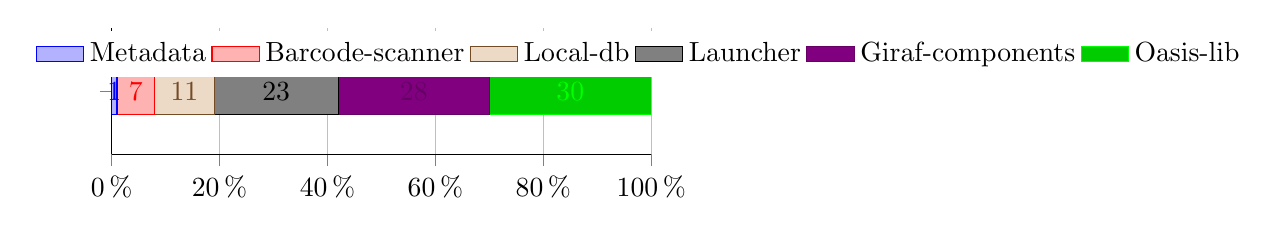
\begin{tikzpicture}
  \begin{axis}[xbar stacked,
axis y line*= none, axis x line*= bottom,
xmajorgrids = true,
ytick = data,
yticklabels = {},
tick align = outside,
xtick pos = left,
bar width=6mm,
y=8mm,
nodes near coords,
xmin=0,
xmax=100,
xticklabel=$\pgfmathprintnumber{\tick}$\,\%,
xticklabel style={/pgf/number format/.cd,fixed,precision=2},
legend style={
  legend columns=-1,
  anchor=north,
  draw=none,
},
area legend,]
    \addplot coordinates
    {(1,0)};
    \addlegendentry{Metadata}
    \addplot coordinates
    {(7,0)};
    \addlegendentry{Barcode-scanner}
    \addplot coordinates
    {(11,0)};
    \addlegendentry{Local-db}
    \addplot coordinates
    {(23,0)};
    \addlegendentry{Launcher}
    \addplot coordinates
    {(28,0)};
    \addlegendentry{Giraf-components}
    \addplot coordinates
    {(30,0)};
    \addlegendentry{Oasis-lib}
  \end{axis}
\end{tikzpicture}